\documentclass{beamer}

\usecolortheme[light]{solarized}

\beamertemplatenavigationsymbolsempty

\usepackage{hyperref}

\usepackage{booktabs}
\usepackage{graphicx}
\usepackage{minted}
\usepackage{moresize}
\usepackage{standalone}
\usepackage{tcolorbox}
\usepackage{tikz}
\usepackage[normalem]{ulem}
\usepackage{xpatch}

\xpatchcmd{\sout}
  {\bgroup}
    {\bgroup\def\ULthickness{2pt}}
      {}{}

\usetikzlibrary{calc, patterns}

\definecolor{twitter}{RGB}{64, 153, 255}
\definecolor{github}{RGB}{211, 211, 211}

\newcommand{\assetsfolder}{./assets}
\newcommand{\researchfolder}{$HOME/rsc/axelrod-moran}
\newcommand{\mlresearchfolder}{$HOME/rsc/ml-paper}
\newcommand{\sseresearchfolder}{$HOME/rsc/testing_for_ZD}

\begin{document}

    \begin{frame}
        \begin{center}
            \Huge
               Vince Knight - \href{https://twitter.com/drvinceknight}{@drvinceknight}\\
        \end{center}
    \end{frame}

    \begin{frame}
        \begin{center}
            \begin{tcolorbox}[colback=twitter,colframe=twitter!40!black,title=
                    \href{https://twitter.com/kirstyjean/status/870415613746962432}
                    {@kirstyjean} (2 Jun 2017):
]
                    Me: sets up flawless heat competition trial, lizards will
                    fight over hot podium, there can only be one winner!

                    Lizards:

                    \#ALlizards2017
           \end{tcolorbox}
        \end{center}
        \begin{center}
            \pause
            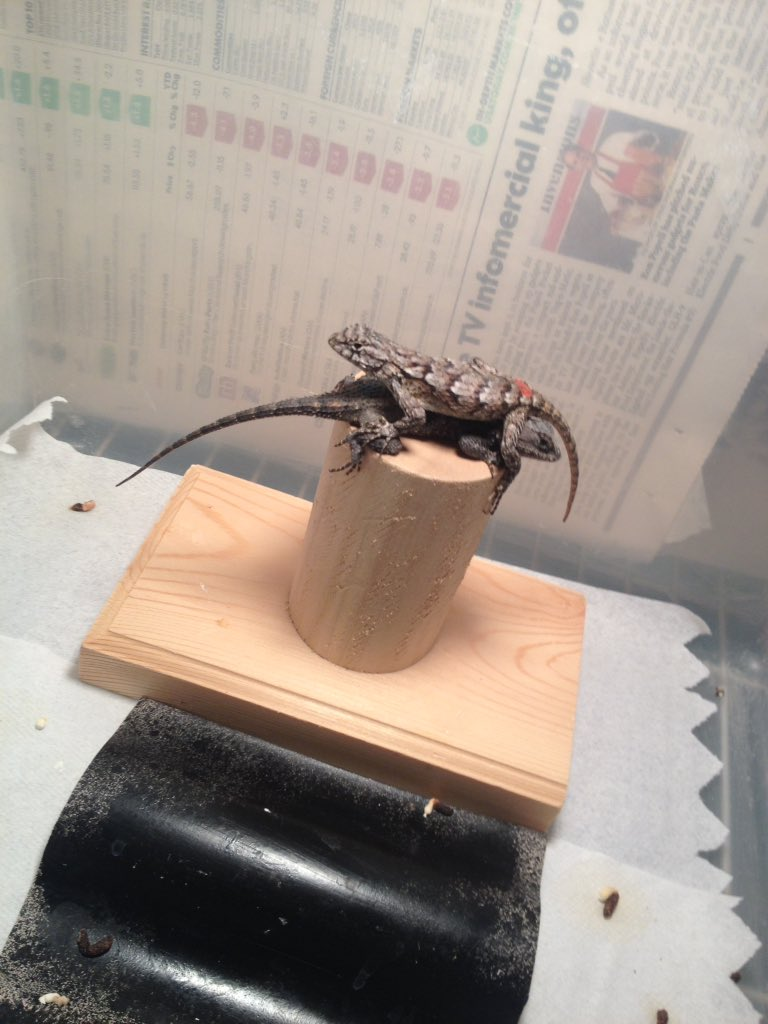
\includegraphics[width=.4\textwidth]
            {\assetsfolder/lizard-cooperation.jpg}
        \end{center}

    \end{frame}

    \begin{frame}
        % PD
        \Huge
        \[
            \begin{pmatrix}
                R & S\\
                T & P
            \end{pmatrix}
            \qquad
            \begin{pmatrix}
                R & T\\
                S & P
            \end{pmatrix}
        \]
    \end{frame}

    \begin{frame}
        % PD
        \Huge
        \[
            \begin{pmatrix}
                3 & 0\\
                5 & 1
            \end{pmatrix}
            \qquad
            \begin{pmatrix}
                3 & 5\\
                0 & 1
            \end{pmatrix}
        \]
    \end{frame}

    \begin{frame}[fragile]{}
        \begin{columns}
            \begin{column}{.4\textwidth}
                \begin{center}
                    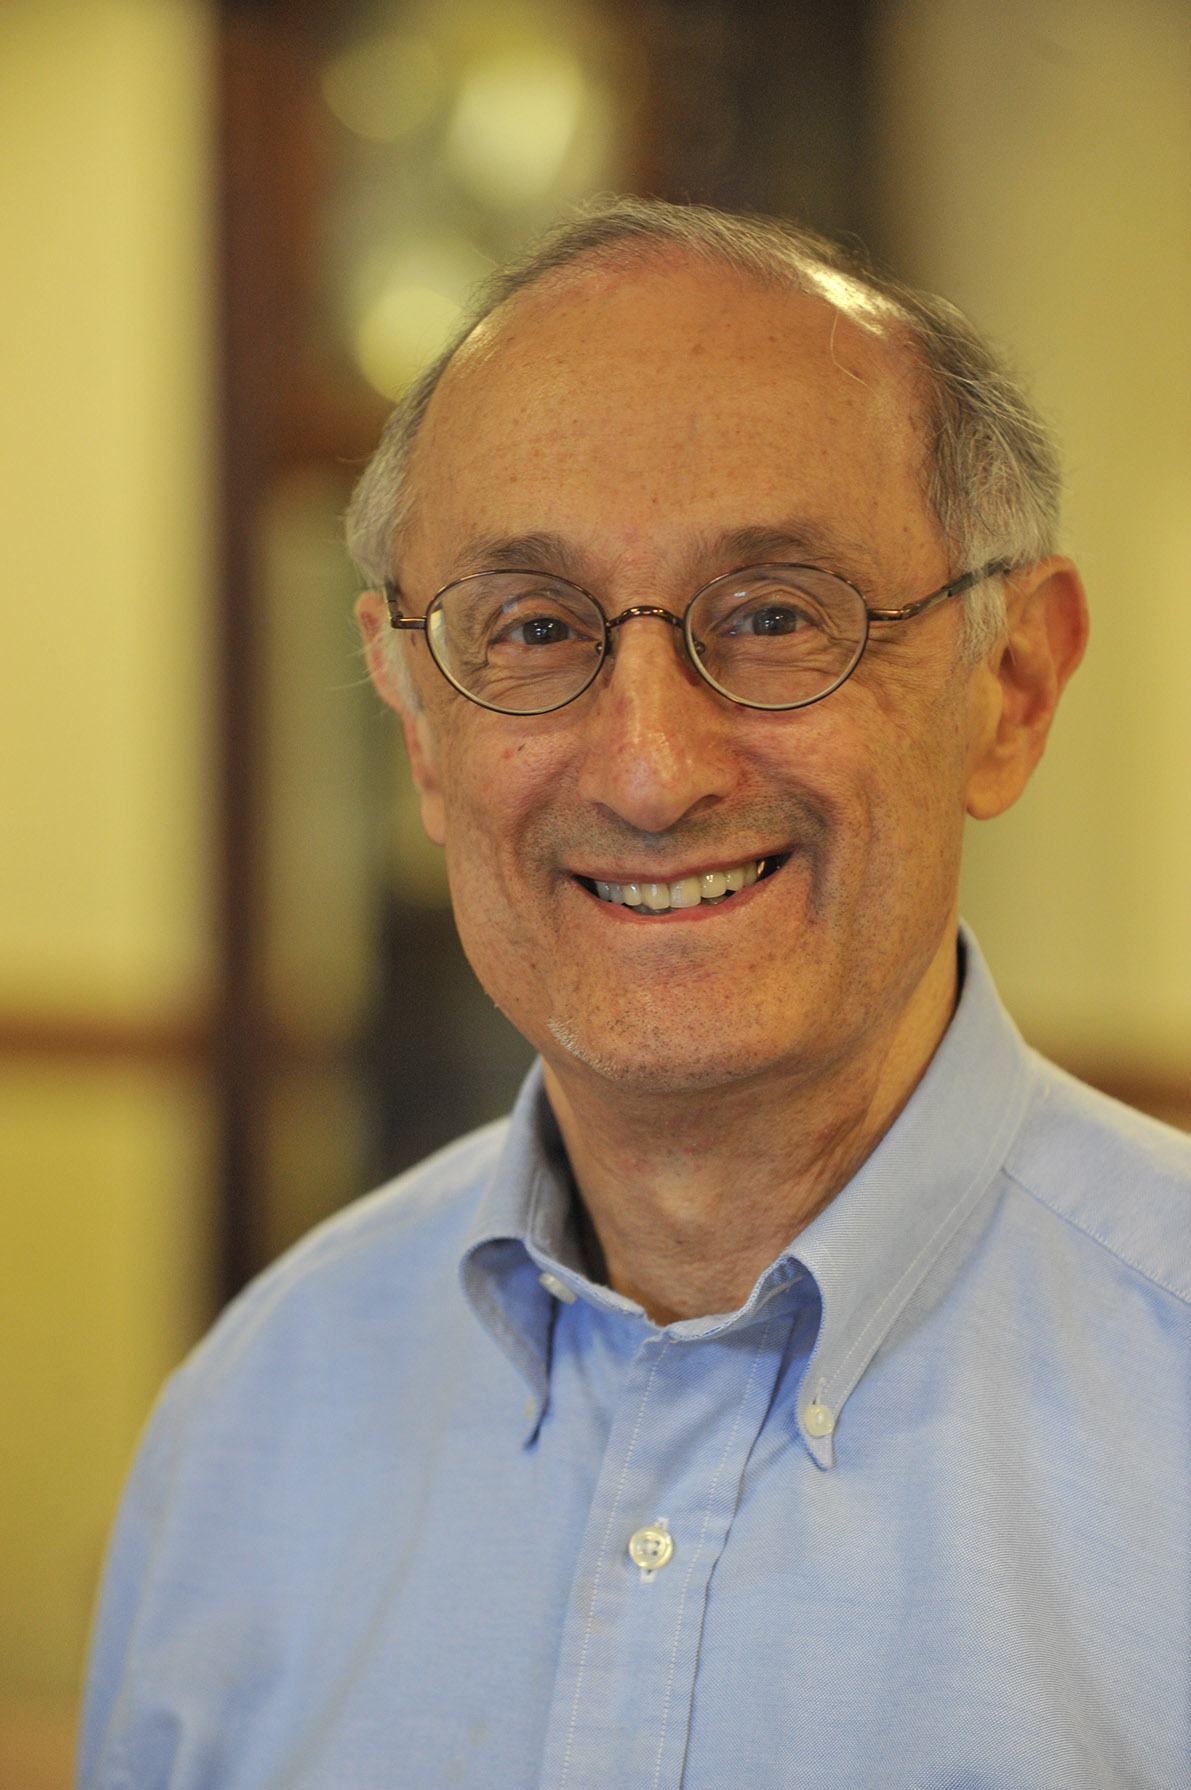
\includegraphics[width=.8\textwidth]{\assetsfolder/Axelrod.jpg}
                    \\
                    Robert Axelrod
                \end{center}
            \end{column}
            \pause
            \begin{column}{.6\textwidth}
                \begin{minted}[fontsize=\scriptsize]{python}
>>> import axelrod as axl

>>> players = (axl.TitForTat(),
...            axl.Cooperator())
>>> axl.Match(players, turns=5).play()
[(C, C), (C, C), (C, C), (C, C), (C, C)]

>>> players = (axl.TitForTat(),
...            axl.Defector())
>>> axl.Match(players, turns=5).play()
[(C, D), (D, D), (D, D), (D, D), (D, D)]

>>> players = (axl.TitForTat(),
...            axl.Alternator())
>>> axl.Match(players, turns=5).play()
[(C, C), (C, D), (D, C), (C, D), (D, C)]

                \end{minted}
            \end{column}
        \end{columns}
\end{frame}

    \begin{frame}
        \begin{center}
            \Huge
            ``Simpler is better''
        \end{center}
    \end{frame}

    \begin{frame}
        \begin{center}
            \Large
            \url{https://github.com/Axelrod-Python/Axelrod}
        \end{center}

        \begin{itemize}
            \item  ``An Open Framework for the Reproducible Study of the Iterated
                Prisoner’s Dilemma.'' - 2016 - Journal of open research software
            \item  ``Reinforcement Learning Produces Dominant Strategies for
                the Iterated Prisoner's Dilemma'' - 2017 - PLOS One
            \item  ``Evolution Reinforces Cooperation with the Emergence of
                Self-Recognition Mechanisms: an empirical study of the Moran
                process for the iterated Prisoner's dilemma'' - 2018 - PLOS One
        \end{itemize}
    \end{frame}

    %\begin{frame}[fragile]{}
        %\begin{center}
            %\begin{minipage}{0.7\textwidth}
                %\begin{minted}[linenos, fontsize=\ssmall]{python}
%def moran(N, game, i=1, seed=0):
    %"""
    %Return the population counts for the Moran process on a game
    %"""
    %population = [0 for _ in range(i)] + [1 for _ in range(N - i)]
    %counts = [(i, N - i)]

    %np.random.seed(seed)

    %while len(set(population)) == 2:

        %scores = []

        %for i, player in enumerate(population):
            %total = 0
            %for j, opponent in enumerate(population):
                %if i != j:
                    %total += game[player, opponent]
            %scores.append(total)

        %total_score = sum(scores)
        %probabilities = [score / total_score for score in scores]
        %reproduce_index = np.random.choice(range(N), p=probabilities)

        %eliminate_index = np.random.randint(N)
        %population[eliminate_index] = population[reproduce_index]

        %counts.append((population.count(0), population.count(1)))
    %return counts
            %\end{minted}
        %\end{minipage}
    %\end{center}
%\end{frame}

    %\begin{frame}[fragile]{}
        %\begin{center}
            %\begin{minipage}{0.7\textwidth}
                %\begin{minted}[linenos, fontsize=\scriptsize, firstnumber=14]{python}
    %for i, player in enumerate(population):
        %total = 0
        %for j, opponent in enumerate(population):
            %if i != j:
                %total += game[player, opponent]
        %scores.append(total)

    %total_score = sum(scores)
    %probabilities = [score / total_score for score in scores]
    %reproduce_index = np.random.choice(range(N), p=probabilities)

    %eliminate_index = np.random.randint(N)
    %population[eliminate_index] = population[reproduce_index]
            %\end{minted}
        %\end{minipage}
    %\end{center}
%\end{frame}


\begin{frame}
    \begin{center}
        \scalebox{.6}{\documentclass{standalone}
\usepackage{tikz}
\usetikzlibrary{calc, shapes, patterns}

\begin{document}
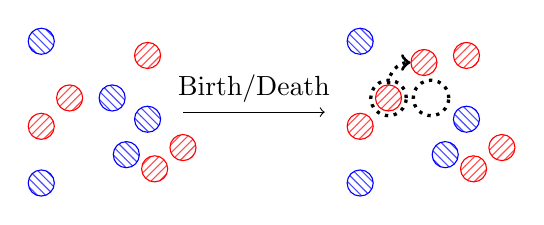
\begin{tikzpicture}[scale=.9]
	\node (A1) at (-1, -1) [circle, pattern=north west lines, pattern
        color=blue!70, draw=blue] {};
	\node (A2) at (-1, 1) [circle, pattern=north west lines, pattern
        color=blue!70, draw=blue] {};
	\node (A3) at (0, .2) [circle, pattern=north west lines, pattern
        color=blue!70, draw=blue] {};
	\node (A4) at (.2, -.6) [circle, pattern=north west lines, pattern
        color=blue!70, draw=blue] {};
	\node (A5) at (.5, -0.1) [circle, pattern=north west lines, pattern
        color=blue!70, draw=blue] {};
	\node (B1) at (-1, -.2) [circle, pattern=north east lines, pattern
        color=red!70, draw=red] {};
	\node (B2) at (1, -.5) [circle, pattern=north east lines, pattern
        color=red!70, draw=red] {};
	\node (B3) at (.5, .8) [circle, pattern=north east lines, pattern
        color=red!70, draw=red] {};
	\node (B4) at (-.6, .2) [circle, pattern=north east lines, pattern
        color=red!70, draw=red] {};
	\node (B5) at (.6, -.8) [circle, pattern=north east lines, pattern
        color=red!70, draw=red] {};

	\draw [->] (1, 0) -- (3, 0) node [above, pos=0.5] {Birth/Death};

	\node (A1) at ($(A1) + (4.5, 0)$) [circle, pattern=north west lines,
        pattern color=blue!70, draw=blue] {};
	\node (A2) at ($(A2) + (4.5, 0)$) [circle, pattern=north west lines,
        pattern color=blue!70, draw=blue] {};
	\node (A3) at ($(A3) + (4.5, 0)$) {};
	\node (A4) at ($(A4) + (4.5, 0)$) [circle, pattern=north west lines,
        pattern color=blue!70, draw=blue] {};
    \node (A5) at ($(A5) + (4.5, 0)$) [circle, pattern=north west lines,
        pattern color=blue!70, draw=blue] {};
	\node (B1) at ($(B1) + (4.5, 0)$) [circle, pattern=north east lines,
        pattern color=red!70, draw=red] {};
	\node (B2) at ($(B2) + (4.5, 0)$) [circle, pattern=north east lines,
        pattern color=red!70, draw=red] {};
	\node (B3) at ($(B3) + (4.5, 0)$) [circle, pattern=north east lines,
        pattern color=red!70, draw=red] {};
	\node (B4) at ($(B4) + (4.5, 0)$) [circle, pattern=north east lines,
        pattern color=red!70, draw=red] {};
	\node (B5) at ($(B5) + (4.5, 0)$) [circle, pattern=north east lines,
        pattern color=red!70, draw=red] {};

	\draw [dotted, very thick] (B4) circle (.25cm);
	\node (B6) at ($(B4) + (0.5, 0.5)$) [circle, pattern=north east lines,
        pattern color=red!70, draw=red] {};
	\draw [->, dotted, very thick] (B4) [out=90, in=180] to (B6);

	\draw [dotted, very thick] (A3) circle (.25cm);
\end{tikzpicture}
\end{document}
}
    \end{center}
\end{frame}


\begin{frame}

    \begin{center}
        \textbf{Resistance}
        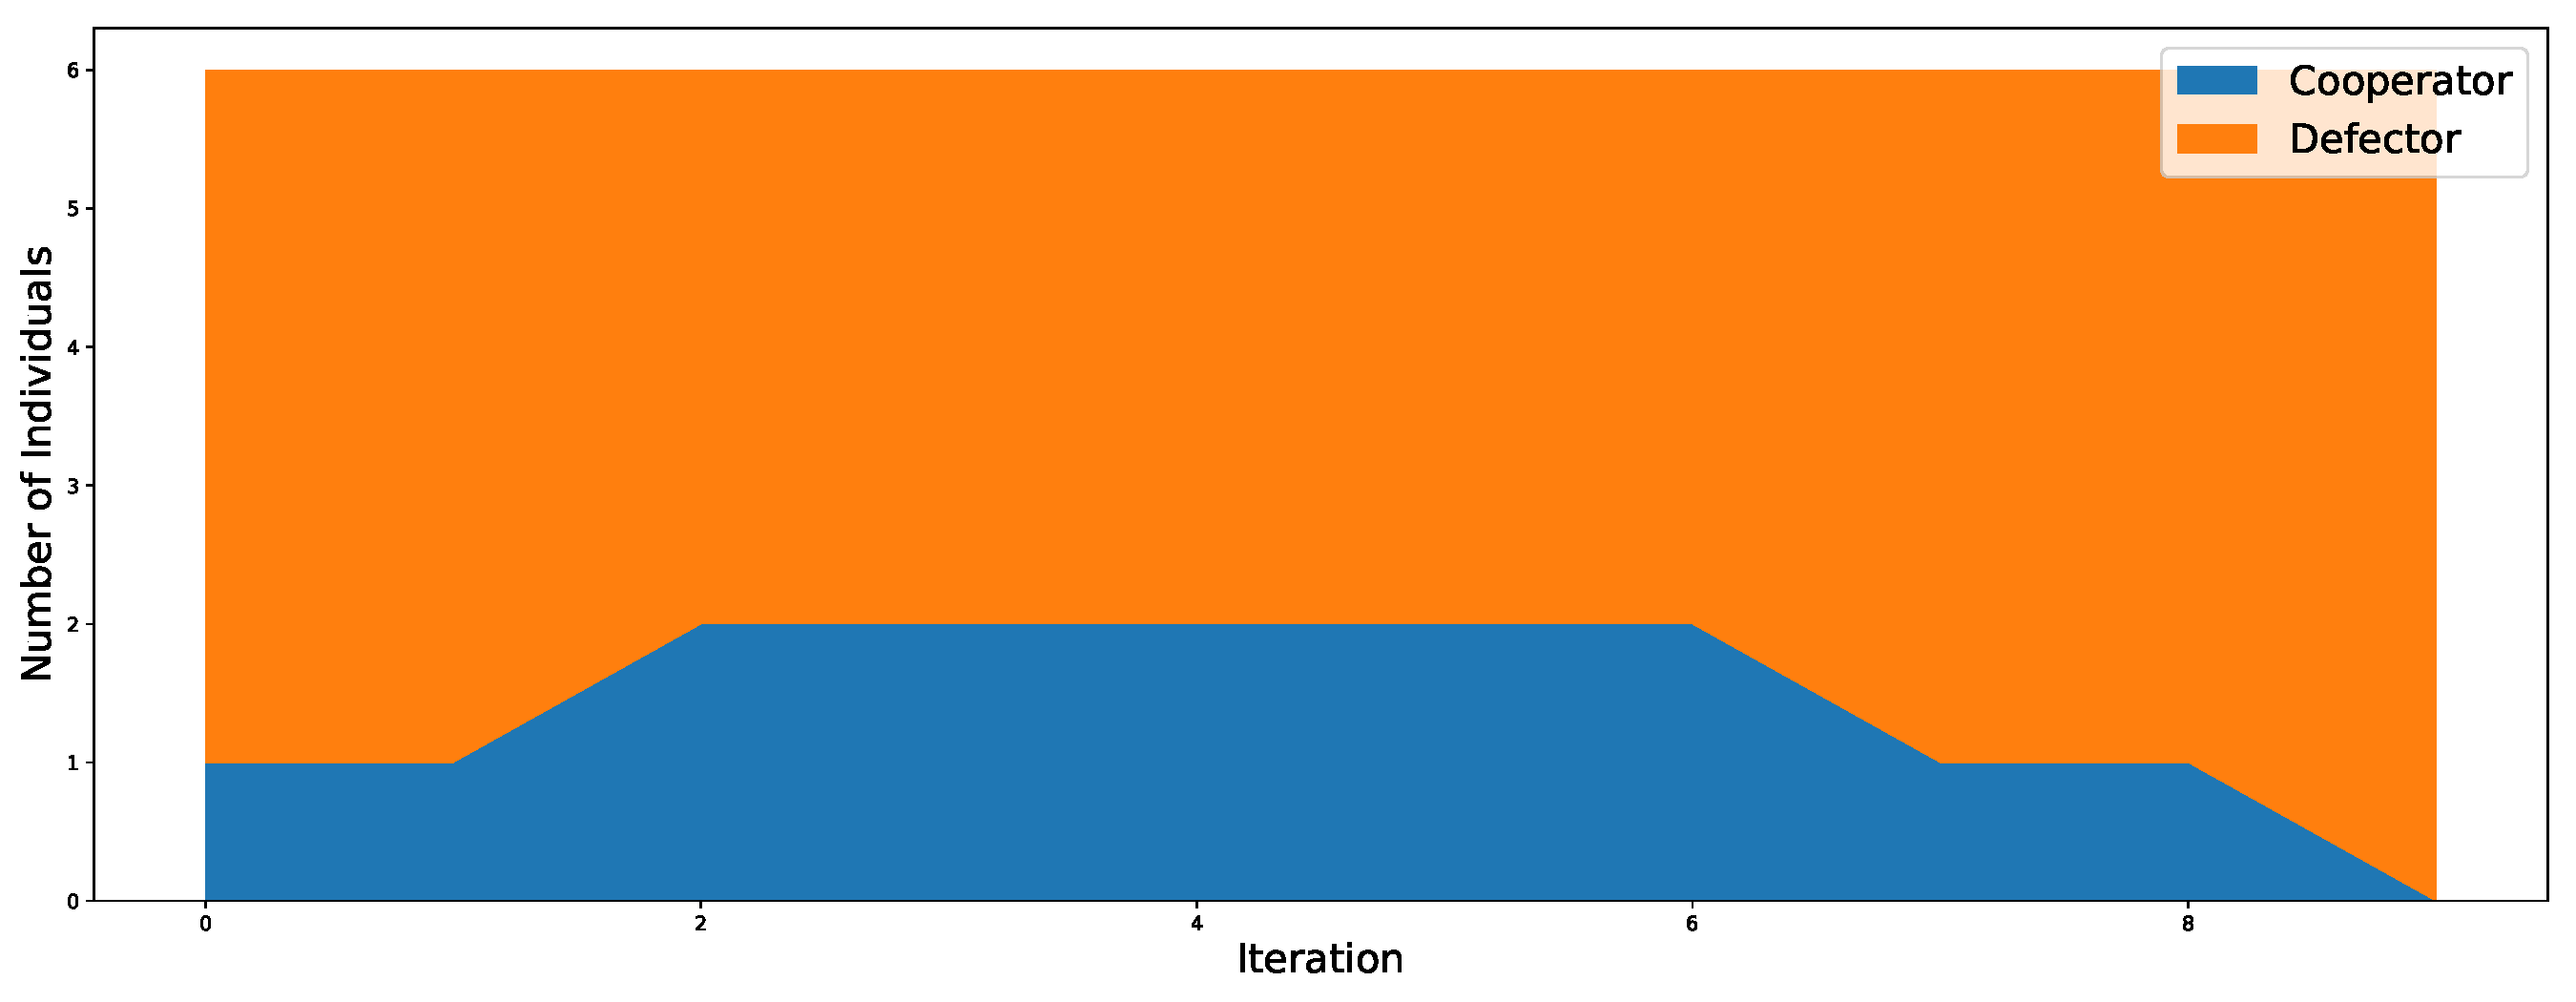
\includegraphics[height=.4\textheight]{\assetsfolder/moran_process_resistance.pdf}\\

        \textbf{Invasion}
        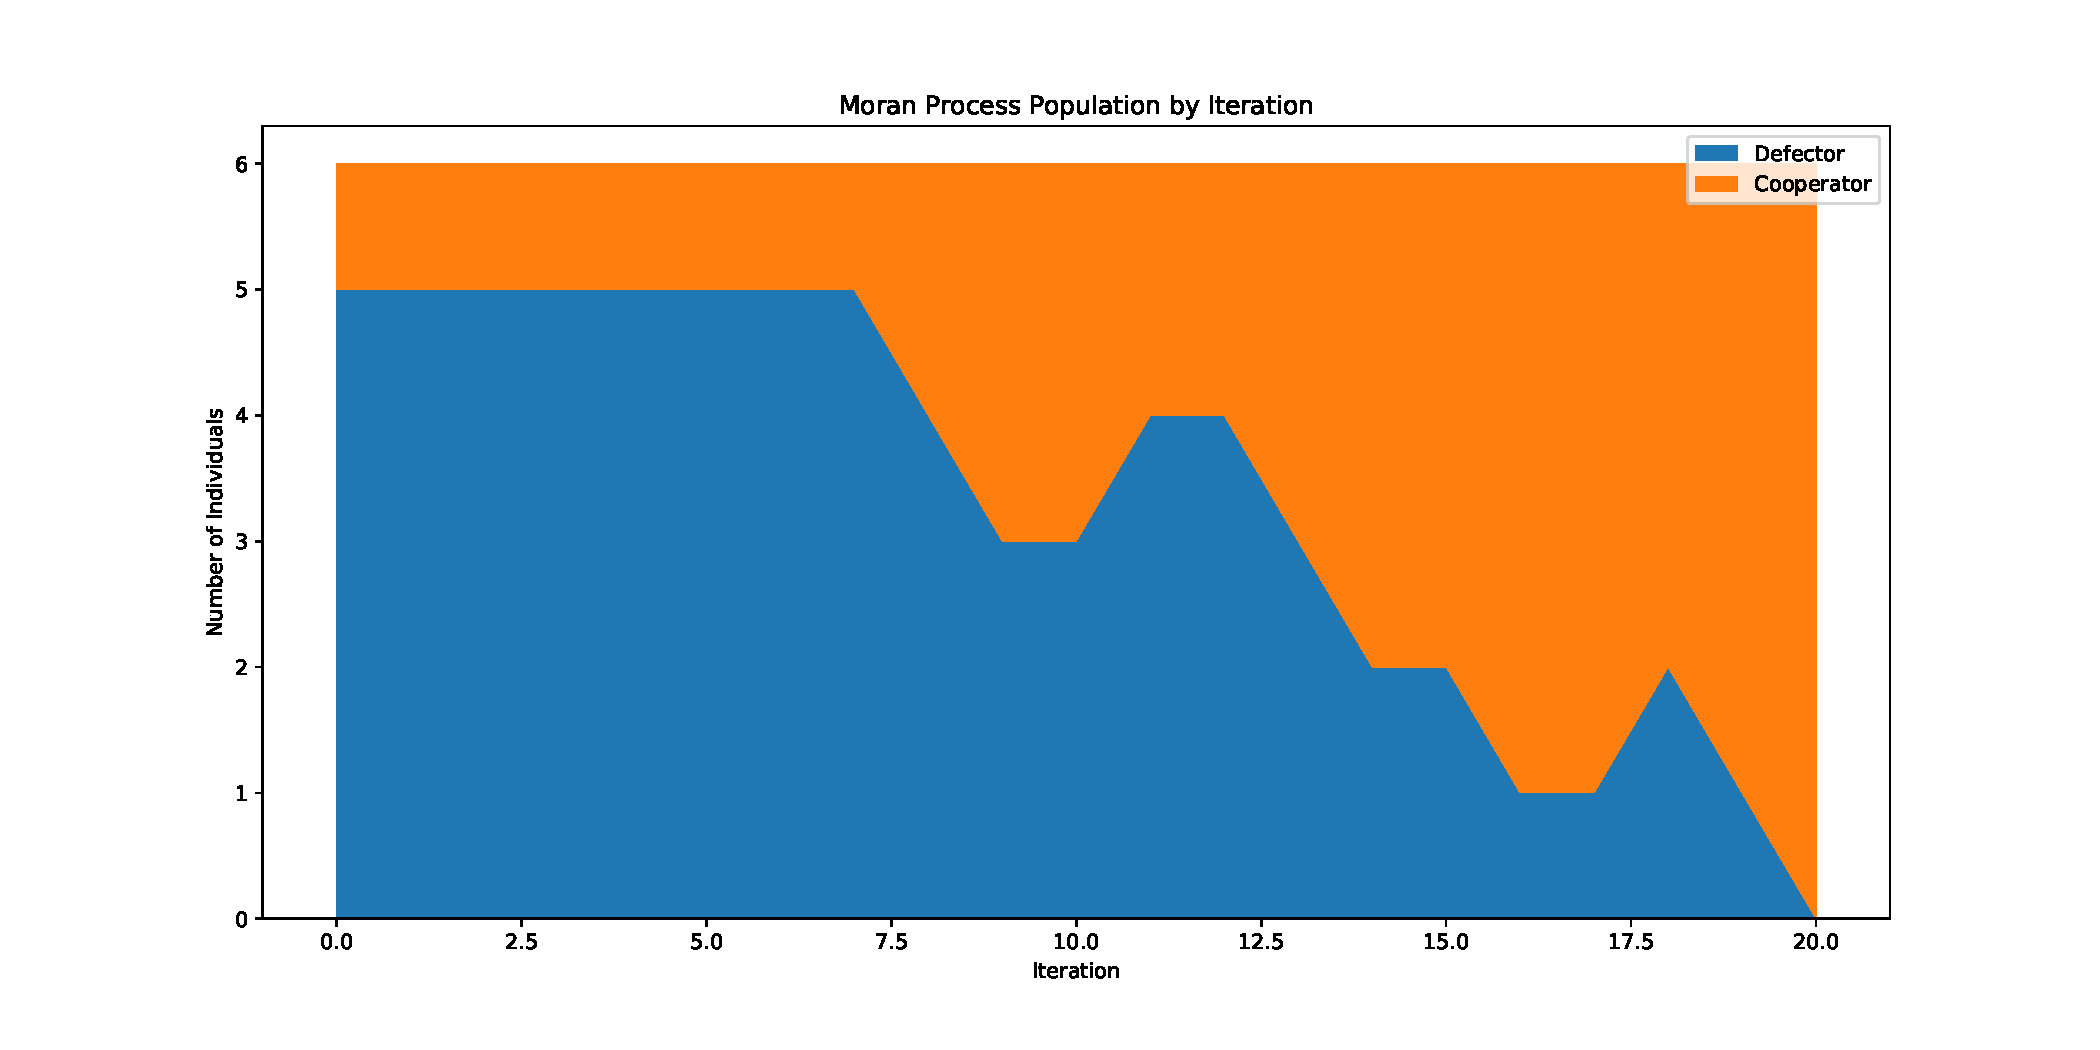
\includegraphics[height=.4\textheight]{\assetsfolder/moran_process_invasion.pdf}
    \end{center}
\end{frame}


\begin{frame}
    \scalebox{.7}{
        \input{\mlresearchfolder/assets/fsm.tex}
    }
\end{frame}

\begin{frame}[fragile]{}

    \begin{center}
        \begin{minipage}{0.8\textwidth}
            \begin{minted}[fontsize=\Huge]{python}
import axelrod_dojo
            \end{minted}
        \end{minipage}
    \end{center}
\end{frame}


\begin{frame}
    \begin{center}
        \scalebox{.7}{
                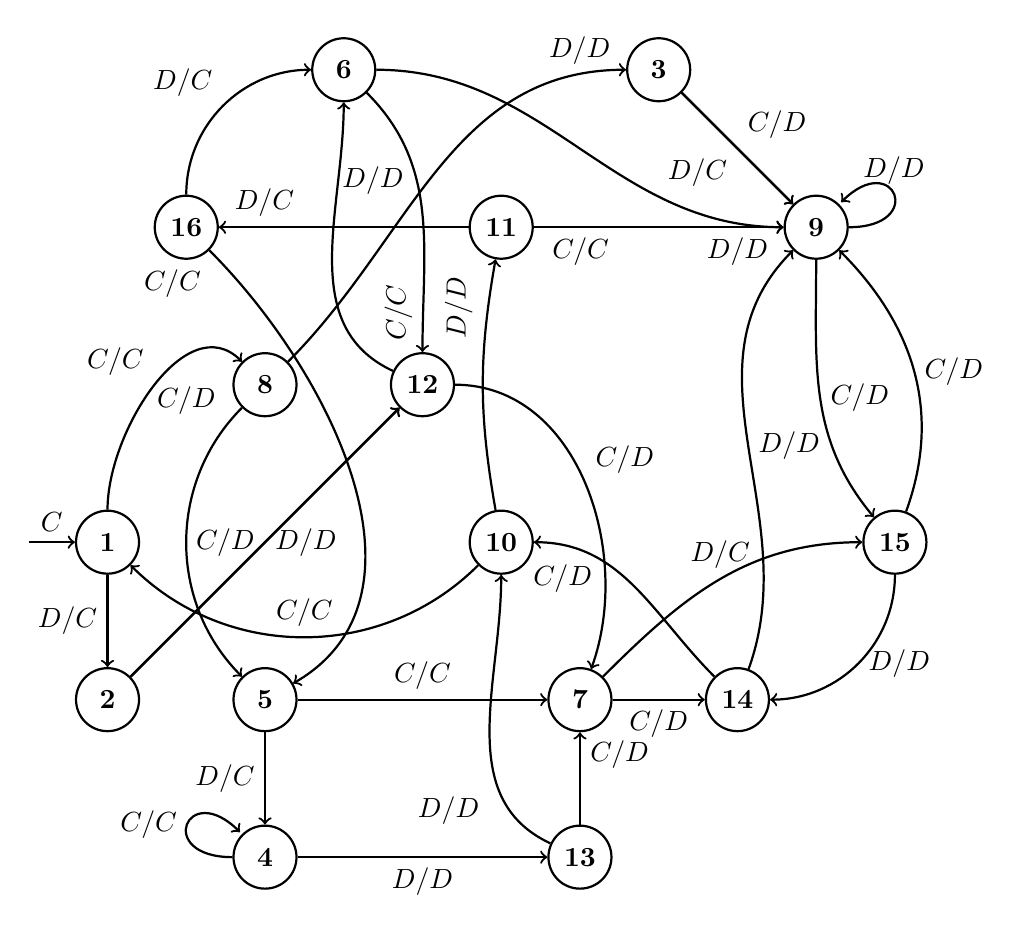
\begin{tikzpicture}

    \tikzstyle{state}=[minimum width=0.8cm, font=\boldmath];
    \node[circle, draw=black, thick] (5) at (0, 0) [state] {$6$};
	\node[circle, draw=black, thick] (2) at (4, 0) [state] {$3$};
	\node[circle, draw=black, thick] (15) at (-2, -2) [state] {$16$};
	\node[circle, draw=black, thick] (8) at ($(2)+(2,-2)$) [state] {$9$};
	\node[circle, draw=black, thick] (10) at ($(15)+(4, 0)$) [state] {$11$};
	
	\node[circle, draw=black, thick] (7) at ($(5)+(-1,-4)$) [state] {$8$};
	\node[circle, draw=black, thick] (11) at ($(7)+(2, 0)$) [state] {$12$};



	\node[circle, draw=black, thick] (9) at ($(10)+(0,-4)$) [state] {$10$};
	\node[circle, draw=black, thick] (0) at ($(9)+(-5,0)$) [state] {$1$};
	\node[circle, draw=black, thick] (14) at ($(9)+(5,0)$) [state] {$15$};

	\node[circle, draw=black, thick] (1) at ($(0)+(0,-2)$) [state] {$2$};
	\node[circle, draw=black, thick] (4) at ($(1)+(2,0)$) [state] {$5$};
	\node[circle, draw=black, thick] (6) at ($(4)+(4,0)$) [state] {$7$};
	\node[circle, draw=black, thick] (13) at ($(6)+(2,0)$) [state] {$14$};

	\node[circle, draw=black, thick] (3) at ($(4)+(0,-2)$) [state] {$4$};
	\node[circle, draw=black, thick] (12) at ($(6)+(0,-2)$) [state] {$13$};


    \coordinate[left of=0] (s);

    \draw (s) edge[out=0, in=180, ->, thick] node [above] {$C$} (0);
    \draw (0) edge[out=90, in=135, ->, thick] node [above left] {$C/C$} (7);
    \draw (0) edge[out=-90, in=90, ->, thick] node [left] {$D/C$} (1);

    \draw (1) edge[out=45, in=-135, ->, thick] node [left] {$C/D$} (11);
    \draw (1) edge[out=45, in=-135, ->, thick] node [right] {$D/D$} (11);
    
    \draw (2) edge[out=-45, in=135, ->, thick] node [above right] {$C/D$} (8);
    \draw (2) edge[out=-45, in=135, ->, thick] node [below left] {$D/C$} (8);

    \draw (3) edge[out=180, in=135, ->, thick, loop] node [left] {$C/C$} (3);
    \draw (3) edge[out=0, in=180, ->, thick] node [below] {$D/D$} (12);

    \draw (4) edge[out=0, in=180, ->, thick] node [above] {$C/C$} (6);
    \draw (4) edge[out=-90, in=90, ->, thick] node [left] {$D/C$} (3);

    \draw (5) edge[out=0, in=180, ->, thick] node [below, yshift=-1cm, xshift=2cm] {$D/D$} (8);
    \draw (5) edge[out=-45, in=90, ->, thick] node [left, yshift=-0.8cm, xshift=-0.3cm, rotate=90] {$C/C$} (11);

    \draw (6) edge[out=0, in=180, ->, thick] node [below] {$C/D$} (13);
    \draw (6) edge[out=45, in=180, ->, thick] node [above] {$D/C$} (14);

    \draw (7) edge[out=-135, in=135, ->, thick] node [yshift=1.8cm] {$C/D$} (4);
    \draw (7) edge[out=45, in=180, ->, thick] node [above, yshift=1.2cm, xshift=1.8cm] {$D/D$} (2);

    \draw (8) edge[out=0, in=45, ->, thick, loop] node [above] {$D/D$} (8);
    \draw (8) edge[out=-90, in=130, ->, thick] node [right] {$C/D$} (14);

    \draw (9) edge[out=-135, in=-45, ->, thick] node [above] {$C/C$} (0);
    \draw (9) edge[out=100, in=-100, ->, thick] node [above left, yshift=1.5cm, rotate=90] {$D/D$} (10);

    \draw (10) edge[out=0, in=180, ->, thick] node [below left, xshift=-0.5cm] {$C/C$} (8);
    \draw (10) edge[out=180, in=0, ->, thick] node [above left, xshift=-0.5cm] {$D/C$} (15);

    \draw (11) edge[out=0, in=70, ->, thick] node [above right] {$C/D$} (6);
    \draw (11) edge[out=155, in=-90, ->, thick] node [right, yshift=1cm] {$D/D$} (5);

    \draw (12) edge[out=90, in=-90, ->, thick] node [above right] {$C/D$} (6);
    \draw (12) edge[out=155, in=-90, ->, thick] node [left, yshift=-1cm] {$D/D$} (9);

    \draw (13) edge[out=135, in=0, ->, thick] node [below left, xshift=-0.4cm, yshift=0.4cm] {$C/D$} (9);
    \draw (13) edge[out=70, in=-135, ->, thick] node [right] {$D/D$} (8);

    \draw (14) edge[out=70, in=-45, ->, thick] node [right] {$C/D$} (8);
    \draw (14) edge[out=-90, in=0, ->, thick] node [right] {$D/D$} (13);

    \draw (15) edge[out=-45, in=30, ->, thick] node [left, xshift=-1.8cm, yshift=2.5cm] {$C/C$} (4);
    \draw (15) edge[out=90, in=180, ->, thick] node [above left] {$D/C$} (5);

    \end{tikzpicture}

        }
    \end{center}
\end{frame}


\begin{frame}
    \begin{center}
        
\includegraphics[height=.8\textheight]{./assets/hunger-games-hand-gesture.eps}


        \tiny
        \vfill
        \flushright{Image made by \url{http://www.freepik.com} from
        \url{https://www.flaticon.com} is licensed by CC BY 3.0}
    \end{center}
\end{frame}


\begin{frame}
    \begin{center}
        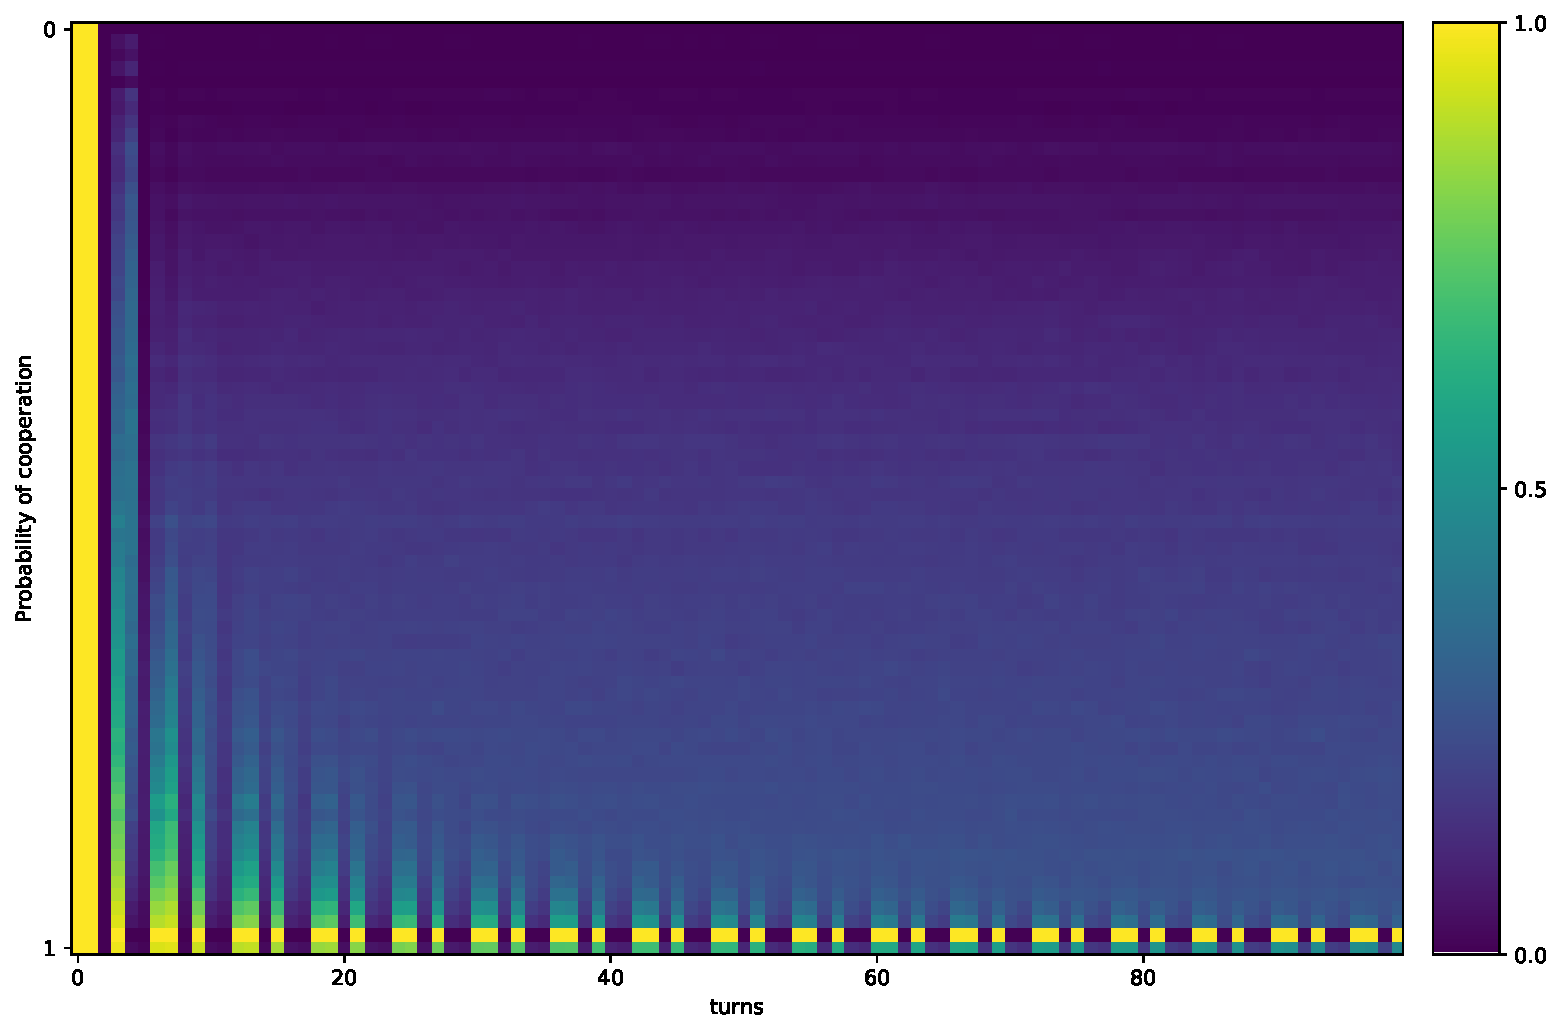
\includegraphics[width=.9\textwidth]{\assetsfolder/tf1_transitive_fingerprint.pdf}
    \end{center}
\end{frame}

\begin{frame}
    \begin{columns}
        \begin{column}{.6\textwidth}
            \begin{center}
                \scalebox{.49}{
                        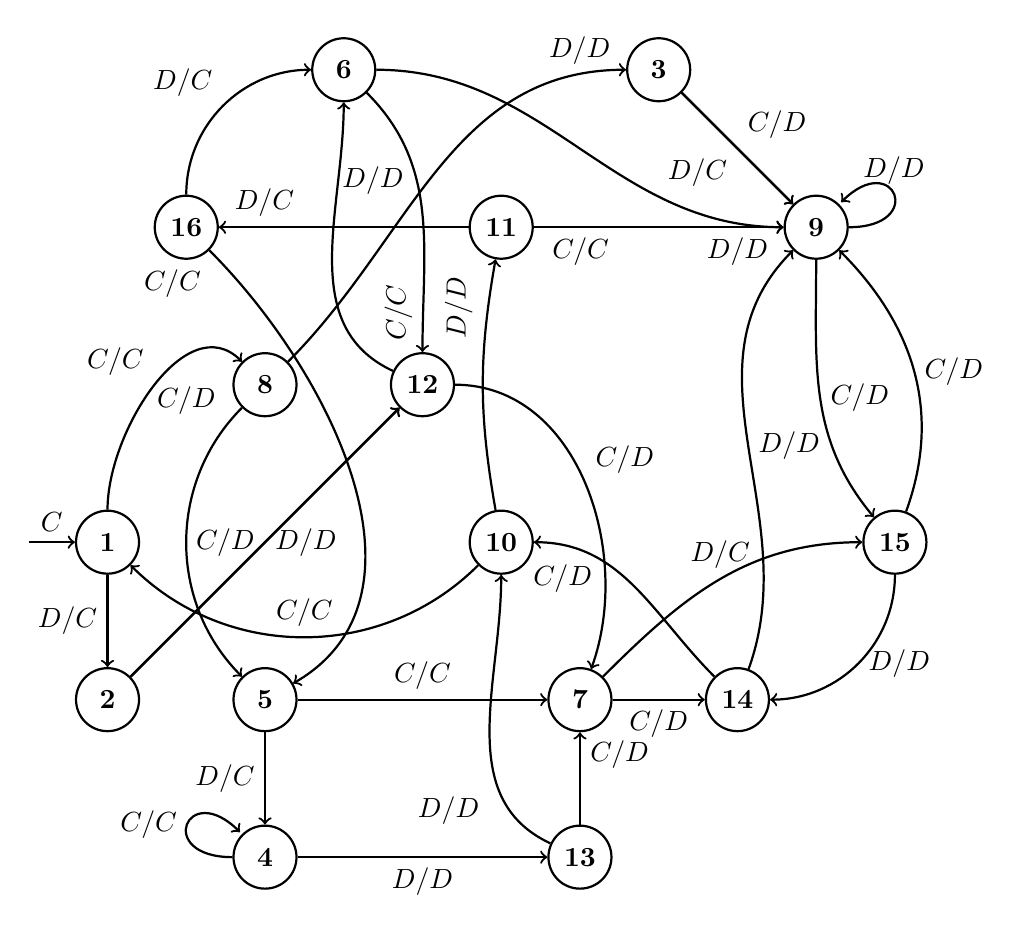
\begin{tikzpicture}

    \tikzstyle{state}=[minimum width=0.8cm, font=\boldmath];
    \node[circle, draw=black, thick] (5) at (0, 0) [state] {$6$};
	\node[circle, draw=black, thick] (2) at (4, 0) [state] {$3$};
	\node[circle, draw=black, thick] (15) at (-2, -2) [state] {$16$};
	\node[circle, draw=black, thick] (8) at ($(2)+(2,-2)$) [state] {$9$};
	\node[circle, draw=black, thick] (10) at ($(15)+(4, 0)$) [state] {$11$};
	
	\node[circle, draw=black, thick] (7) at ($(5)+(-1,-4)$) [state] {$8$};
	\node[circle, draw=black, thick] (11) at ($(7)+(2, 0)$) [state] {$12$};



	\node[circle, draw=black, thick] (9) at ($(10)+(0,-4)$) [state] {$10$};
	\node[circle, draw=black, thick] (0) at ($(9)+(-5,0)$) [state] {$1$};
	\node[circle, draw=black, thick] (14) at ($(9)+(5,0)$) [state] {$15$};

	\node[circle, draw=black, thick] (1) at ($(0)+(0,-2)$) [state] {$2$};
	\node[circle, draw=black, thick] (4) at ($(1)+(2,0)$) [state] {$5$};
	\node[circle, draw=black, thick] (6) at ($(4)+(4,0)$) [state] {$7$};
	\node[circle, draw=black, thick] (13) at ($(6)+(2,0)$) [state] {$14$};

	\node[circle, draw=black, thick] (3) at ($(4)+(0,-2)$) [state] {$4$};
	\node[circle, draw=black, thick] (12) at ($(6)+(0,-2)$) [state] {$13$};


    \coordinate[left of=0] (s);

    \draw (s) edge[out=0, in=180, ->, thick] node [above] {$C$} (0);
    \draw (0) edge[out=90, in=135, ->, thick] node [above left] {$C/C$} (7);
    \draw (0) edge[out=-90, in=90, ->, thick] node [left] {$D/C$} (1);

    \draw (1) edge[out=45, in=-135, ->, thick] node [left] {$C/D$} (11);
    \draw (1) edge[out=45, in=-135, ->, thick] node [right] {$D/D$} (11);
    
    \draw (2) edge[out=-45, in=135, ->, thick] node [above right] {$C/D$} (8);
    \draw (2) edge[out=-45, in=135, ->, thick] node [below left] {$D/C$} (8);

    \draw (3) edge[out=180, in=135, ->, thick, loop] node [left] {$C/C$} (3);
    \draw (3) edge[out=0, in=180, ->, thick] node [below] {$D/D$} (12);

    \draw (4) edge[out=0, in=180, ->, thick] node [above] {$C/C$} (6);
    \draw (4) edge[out=-90, in=90, ->, thick] node [left] {$D/C$} (3);

    \draw (5) edge[out=0, in=180, ->, thick] node [below, yshift=-1cm, xshift=2cm] {$D/D$} (8);
    \draw (5) edge[out=-45, in=90, ->, thick] node [left, yshift=-0.8cm, xshift=-0.3cm, rotate=90] {$C/C$} (11);

    \draw (6) edge[out=0, in=180, ->, thick] node [below] {$C/D$} (13);
    \draw (6) edge[out=45, in=180, ->, thick] node [above] {$D/C$} (14);

    \draw (7) edge[out=-135, in=135, ->, thick] node [yshift=1.8cm] {$C/D$} (4);
    \draw (7) edge[out=45, in=180, ->, thick] node [above, yshift=1.2cm, xshift=1.8cm] {$D/D$} (2);

    \draw (8) edge[out=0, in=45, ->, thick, loop] node [above] {$D/D$} (8);
    \draw (8) edge[out=-90, in=130, ->, thick] node [right] {$C/D$} (14);

    \draw (9) edge[out=-135, in=-45, ->, thick] node [above] {$C/C$} (0);
    \draw (9) edge[out=100, in=-100, ->, thick] node [above left, yshift=1.5cm, rotate=90] {$D/D$} (10);

    \draw (10) edge[out=0, in=180, ->, thick] node [below left, xshift=-0.5cm] {$C/C$} (8);
    \draw (10) edge[out=180, in=0, ->, thick] node [above left, xshift=-0.5cm] {$D/C$} (15);

    \draw (11) edge[out=0, in=70, ->, thick] node [above right] {$C/D$} (6);
    \draw (11) edge[out=155, in=-90, ->, thick] node [right, yshift=1cm] {$D/D$} (5);

    \draw (12) edge[out=90, in=-90, ->, thick] node [above right] {$C/D$} (6);
    \draw (12) edge[out=155, in=-90, ->, thick] node [left, yshift=-1cm] {$D/D$} (9);

    \draw (13) edge[out=135, in=0, ->, thick] node [below left, xshift=-0.4cm, yshift=0.4cm] {$C/D$} (9);
    \draw (13) edge[out=70, in=-135, ->, thick] node [right] {$D/D$} (8);

    \draw (14) edge[out=70, in=-45, ->, thick] node [right] {$C/D$} (8);
    \draw (14) edge[out=-90, in=0, ->, thick] node [right] {$D/D$} (13);

    \draw (15) edge[out=-45, in=30, ->, thick] node [left, xshift=-1.8cm, yshift=2.5cm] {$C/C$} (4);
    \draw (15) edge[out=90, in=180, ->, thick] node [above left] {$D/C$} (5);

    \end{tikzpicture}

                }
            \end{center}
        \end{column}

        \begin{column}{.4\textwidth}
            \small
            \begin{tabular}{ll}
                \toprule
                TF1 \#1   & TF1 \#2\\
                \midrule
                \bf{1}: C & \bf{1}: C  \\
                \bf{8}: C & \bf{8}: C  \\
                \bf{5}: D & \bf{5}: D  \\
                4: C      & 4: C  \\
                4: C      & 4: C  \\
                4: C      & 4: C  \\
                4: C      & 4: C  \\
                4: C      & 4: C  \\
                \bottomrule
            \end{tabular}
        \end{column}
    \end{columns}
\end{frame}

\begin{frame}
    \begin{center}
        \Huge ``Don't trust anyone.''
    \end{center}
\end{frame}

\begin{frame}
    \begin{center}
        \Large \textbf{Press and Dyson} 2012: ``Iterated Prisoner’s Dilemma contains
        strategies that dominate any evolutionary opponent''
    \end{center}
\end{frame}

\begin{frame}
    \begin{center}
        \Large``The world of game theory is currently on fire.''
    \end{center}
    \begin{flushright}
        MIT Technology Review, 2012
    \end{flushright}
\end{frame}

\begin{frame}
	\begin{center}
		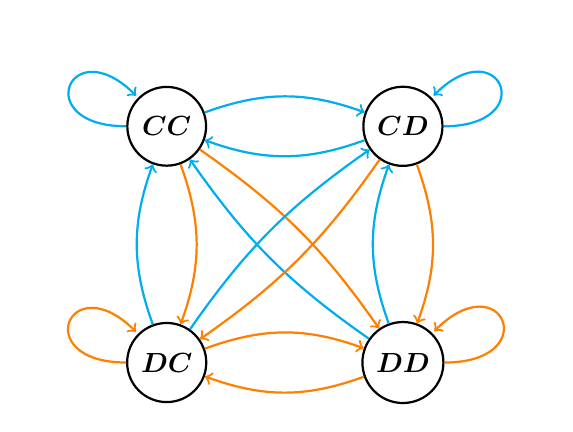
\begin{tikzpicture}
			\tikzstyle{state}=[minimum width=1cm, font=\boldmath];

			\node[circle, draw, thick] (0) at (0, 0) [state] {$CC$};
			\node[circle, draw, thick] (1) at (3, 0) [state] {$CD$};
			\node[circle, draw, thick] (2) at (0, -3) [state] {$DC$};
			\node[circle, draw, thick] (3) at (3, -3) [state] {$DD$};

			\draw (0) edge[cyan,out=20, in=160, ->, thick] node [above] {} (1);
			\draw (1) edge[cyan, out=-160, in=-20, ->, thick] node [above] {} (0);

			\draw (2) edge[orange,out=20, in=160, ->, thick] node [above] {} (3);
			\draw (3) edge[orange, out=-160, in=-20, ->, thick] node [above] {} (2);

			\draw (0) edge[orange,out=-70, in=70, ->, thick] node [above] {} (2);
			\draw (2) edge[cyan, out=110, in=-110, ->, thick] node [above] {} (0);

			\draw (1) edge[orange,out=-70, in=70, ->, thick] node [above] {} (3);
			\draw (3) edge[cyan, out=110, in=-110, ->, thick] node [above] {} (1);

			\draw (0) edge[orange,out=-35, in=125, ->, thick] node [above] {} (3);
			\draw (3) edge[cyan, out=145, in=-55, ->, thick] node [above] {} (0);

			\draw (1) edge[orange,out=-125, in=35, ->, thick] node [above] {} (2);
			\draw (2) edge[cyan, out=55, in=-145, ->, thick] node [above] {} (1);

			\draw (0) edge[cyan, out=180, in=135, ->, thick, loop] node [above] {}  (0);
			\draw (2) edge[orange,out=180, in=135, ->, thick, loop] node [above] {} (2);

			\draw (1) edge[cyan,out=0, in=45, ->, thick, loop] node [above] {} (1);
			\draw (3) edge[orange, out=0, in=45, ->, thick, loop] node [above] {} (3);

		\end{tikzpicture}
    \end{center}
\end{frame}

\begin{frame}

If

\begin{equation}\label{eqn:linear_relationship_for_p}
    \tilde p=\alpha S_x + \beta S_y + \gamma
\end{equation}

then:

\begin{equation}
    \alpha S_X + \beta S_Y + \gamma = 0
\end{equation}

Specifically:

\begin{equation}
    S_X = -\frac{\beta}{\alpha} S_Y = \chi S_y
\end{equation}
\end{frame}

\begin{frame}
    \begin{center}
        \Huge
        ``Extortion cannot be beaten.''
    \end{center}
\end{frame}

\begin{frame}
    \Large
    \begin{align}
    \tilde p_1 & = \alpha R + \beta R - P (\alpha + \beta)
            \label{eqn:condition_for_tilde_p1}\\
    \tilde p_2 & = \alpha S + \beta T - P (\alpha + \beta)
            \label{eqn:condition_for_tilde_p2}\\
    \tilde p_3 & = \alpha T + \beta S - P (\alpha + \beta)
            \label{eqn:condition_for_tilde_p3}\\
    \tilde p_4 & = \alpha P + \beta P - P (\alpha + \beta) = 0
            \label{eqn:condition_for_tilde_p4}
    \end{align}

    with:

    \begin{equation}\label{eqn:definition_of_chi}
        \chi = \frac{\tilde p_2 (P - T) + \tilde p_3 (S - P)}
                    {\tilde p_2 (P - S) + \tilde p_3 (T - P)}
    \end{equation}
\end{frame}

\begin{frame}
    \Large
    \begin{equation}\label{eqn:linear_algebraic_equation_for_p}
        Cx= \tilde p
    \end{equation}

    \begin{equation}\label{eqn:definition_of_C}
        C =
        \begin{bmatrix}
            R - P & R- P \\
            S - P & T- P \\
            T - P & S- P \\
            0     & 0 \\
        \end{bmatrix}
    \end{equation}
\end{frame}

\begin{frame}
    \Large
    \begin{equation}\label{eqn:x_star}
        x^* = \text{argmin}_{x\in\mathbb{R}^2}\|C x- p^*\|_2^2
    \end{equation}

    \begin{equation}\label{eqn:x_SSError_formula}
        \text{SSE} = {p ^ *} ^ T p ^ * -
               p ^ * C \left(C ^ T C \right) ^ {-1} C ^ T p ^ *
             = {p ^ *} ^ T p ^ * - p ^ * C x ^ *
    \end{equation}

\end{frame}

\begin{frame}
    \begin{center}
    
\includegraphics[width=.8\textwidth]{\sseresearchfolder/assets/img/sse_chi_probabilities_in_full/main.pdf}
    \end{center}
\end{frame}

\begin{frame}
    \begin{center}
        
\includegraphics[width=\textwidth]{\sseresearchfolder/assets/img/replicator_dynamics/main.pdf}
    \end{center}
\end{frame}

\begin{frame}
    \begin{center}
    
\includegraphics[width=\textwidth]{\sseresearchfolder/assets/img/compare-evolutionary-dynamics-to-sserror/main.pdf}
    \end{center}
\end{frame}

\begin{frame}
    \begin{table}[!hbtp]
        \begin{center}
        \tiny
        \documentclass{beamer}

\usecolortheme[light]{solarized}

\beamertemplatenavigationsymbolsempty

\usepackage{hyperref}

\usepackage{tikz}
\usetikzlibrary{calc}

\begin{document}

\begin{center}


    \begin{tikzpicture}
        \draw [thick] (0,-4) -- (0, 4);
        \draw [thick] (-5,0) -- (5, 0);

        \node at (-2, 2) {Tutorials};
        \node at (2, 2) {How To's};
        \node at (-2, -2) {Discussions};
        \node at (2, -2) {Reference};
    \end{tikzpicture}

\href{"https://twitter.com/evildmp"}{@EVILDMP}

\end{center}



\end{document}

        \end{center}
    \end{table}
\end{frame}

\begin{frame}
    \Large
    \begin{quote}
        ``It is not the most intellectual of the species that survives; it is not the
        strongest that survives; but the species that survives is the one that is able
        to adapt to and to adjust best to the changing environment in which it finds
        itself.''
    \end{quote}
    \pause
    \begin{flushright}
        Darwin.
    \end{flushright}
\end{frame}

\begin{frame}
    \begin{footnotesize}
        \begin{tcolorbox}[colback=github,colframe=blue!40!black,title=
                Julie Rymer - \href{https://gitter.im/Axelrod-Python/Axelrod?at=591388592b926f8a6741435d}
                {@Chadys} - (10 May 2017):
    ]
                And I really wanted to thank you all, I discovered your project because of a
                course where we needed to participate in an open source project, and I had the
                occasion to compare the welcome me and my coworkers received here compared to
                other people from my class who worked on different project. And I've got to said
                you are awesome on that part and on the help your provide to newbies  I like
                your project so I'll try to continue to contribute now and then !
       \end{tcolorbox}
    \end{footnotesize}

   \begin{columns}
        \begin{column}{.35\textwidth}
            \begin{itemize}
                \item \href{https://twitter.com/NikoletaGlyn}{@NikoletaGlyn}
                \item \href{https://twitter.com/opcampbell}{@opcampbell}
                \item \href{http://marcharper.codes/}{marcharper.codes}
                \item \href{https://www.cardiff.ac.uk/people/view/98648-gillard-jonathan}{Jonathan Gillard}
            \end{itemize}
        \end{column}
        \begin{column}{.65\textwidth}
            \begin{itemize}
                \item \href{https://github.com/Axelrod-Python/Axelrod}{github.com/Axelrod-Python/Axelrod}
                \item \href{https://gitter.im/Axelrod-Python/Axelrod}{gitter.im/Axelrod-Python/Axelrod}
                \item
                    \href{https://arxiv.org/abs/1707.06920}{arxiv.org/abs/1707.06920}
            \end{itemize}
        \end{column}
   \end{columns}

        \begin{center}
               \href{https://twitter.com/drvinceknight}{@drvinceknight}
        \end{center}

   \begin{columns}
        \begin{column}{.4\textwidth}
            \begin{itemize}
                \item
                    \href{https://vknight.org/gt/}{vknight.org/gt/}
            \end{itemize}
        \end{column}
        \begin{column}{.6\textwidth}
            \begin{itemize}
                \item \href{https://github.com/drvinceknight/Nashpy}{github.com/drvinceknight/Nashpy}
            \end{itemize}
        \end{column}
   \end{columns}
\end{frame}


\end{document}
